
\chapter{Application Description}

In this chapter present the application using code snippets, diagrams.

\section{Architecture}

The application uses an Event Driven architecture, making as much use as possible of Node JS's built in capabilities for handling multiple operations on a single thread using concurrency and asynchronous programming.

The application consists of multiple microservices, all comunicating using Rabbit MQ. The microservices used are:
\begin{itemize}
    \item Client - User interface, hosted on a server of its own.
    \item Authentication Service - RPC server, handling all authentication logic.
    \item Core BZL Service - RPC server, handling all other computations, data proessing and access to the database.
    \item User Service - HTTP server, accepting reguests relating to users, and sending an event to the Core bzl or Auth Services in order for them to process the data.
    \item File Uploader Service - HTTP server, accepting reguests relating to file management, and sending an event to the Core BZL Service in order for it to process the data.
    \item Chat Service - HTTP server, using web sockets, that handles all chat related data.
\end{itemize}

Authentication Logic (e.g. Figure \ref{fig:authLogic}).

File upload Logic (e.g Figure \ref{fig:uploaderLogic}).

Use Case Diagram (e.g Figure \ref{fig:useCase}).
\begin{figure}[!ht]
    \centering
    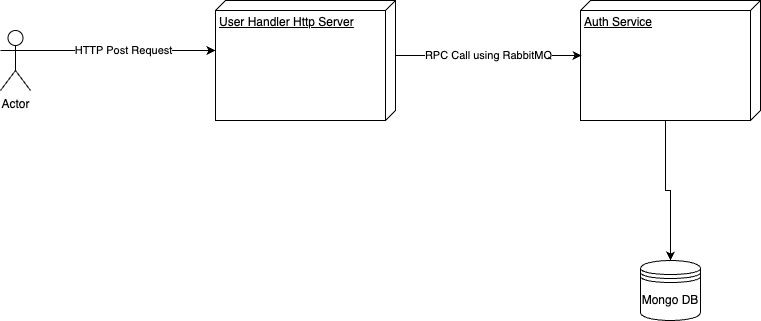
\includegraphics[width=1\linewidth]{Ples Serban Thesis/login.drawio.png}
    \caption{Authentication Logic Diagram}
    \label{fig:authLogic}
\end{figure}

\begin{figure}[!ht]
    \centering
    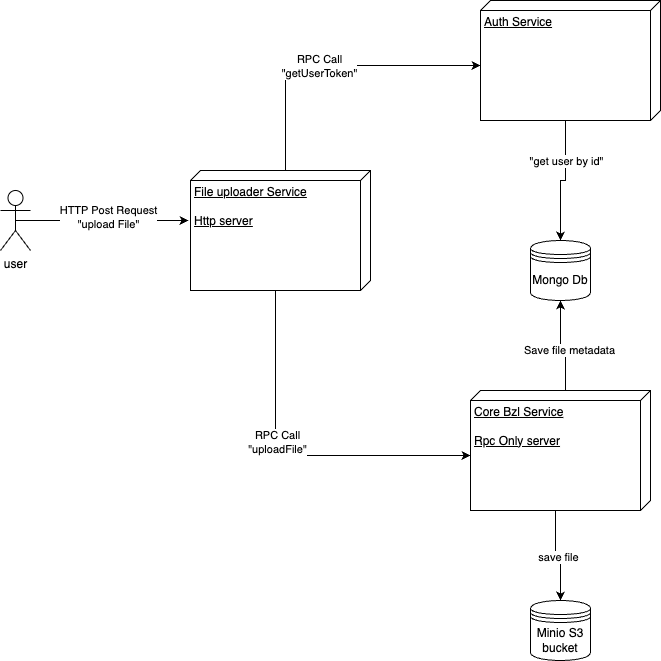
\includegraphics[width=1\linewidth]{Ples Serban Thesis/file uplaod.drawio.png}
    \caption{File Uploader Logic Diagram}
    \label{fig:uploaderLogic}
\end{figure}

\begin{figure}[!ht]
    \centering
    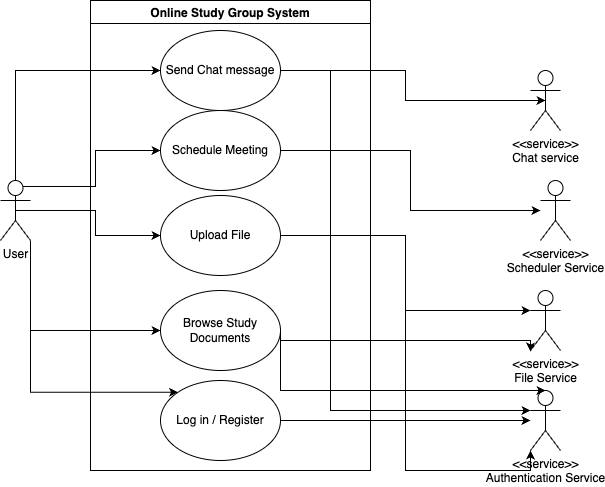
\includegraphics[width=1\linewidth]{Ples Serban Thesis/Use Case Licenta.drawio.png}
    \caption{Use Case Diagram}
    \label{fig:useCase}
\end{figure}

\newpage
\section{Features}
Present all of the features.

\section{Technology Stack}
Present information on the technologies used:
\begin{defn} Angular
\end{defn}
\begin{defn} Node JS
\end{defn}
\begin{defn} Minio S3
\end{defn}
\begin{defn} Mongo DB
\end{defn}
\begin{defn} Rabbit MQ
\end{defn}

\section{References}
The bibliography has to be referenced in thesis content using cite (e.g. \cite{Bersani}).

\section{Interface}
Present App interface using Screenshots?

Each figure has to have a caption that is a suggestive description of what  the  picture represents (e.g. Figure \ref{fig:siglaUVT}).
\begin{figure}[!ht]
    \centering
    
\includegraphics[width=0.25\linewidth]{Ples Serban Thesis/FMI-03.png}
    \caption{ FMI logo scaled at 25\% of text width}
    \label{fig:siglaUVT}
\end{figure}

\section{Algorithm pseudo-code}
Present pseudo-code and actual code for a feature.

Pseudo-code is a formal way to describe an algorithm, is more clear than a textual description ore code ( e.g. Algorithn \ref{alg:alg_ex}).

\begin{algorithm}[!ht]
\caption{An algorithm with caption}\label{alg:alg_ex}
\begin{algorithmic}[1]
\Require $n \geq 0$
\Ensure $y = x^n$
\State $y \gets 1$
\State $X \gets x$
\State $N \gets n$
\While{$N \neq 0$}
\If{$N$ is even}
    \State $X \gets X \times X$
    \State $N \gets \frac{N}{2}$  \Comment{This is a comment}
\ElsIf{$N$ is odd}
    \State $y \gets y \times X$
    \State $N \gets N - 1$
\EndIf
\EndWhile
\end{algorithmic}
\end{algorithm}

\section{Adding code}
If it necessary to add  some code from the application, do not use print-screens, use  listing  (e.g. listing \ref{lst:p1}).
\begin{lstlisting}[language=Python, numbers=left,
    stepnumber=1, caption=Un exemplu de cod python, label=lst:p1]
import numpy as np
    
def incmatrix(genl1,genl2):
    m = len(genl1)
    n = len(genl2)
    M = None #to become the incidence matrix
    VT = np.zeros((n*m,1), int)  #dummy variable
    
    #compute the bitwise xor matrix
    M1 = bitxormatrix(genl1)
    M2 = np.triu(bitxormatrix(genl2),1) 

    for i in range(m-1):
        for j in range(i+1, m):
            [r,c] = np.where(M2 == M1[i,j])
            for k in range(len(r)):
                VT[(i)*n + r[k]] = 1;
                VT[(i)*n + c[k]] = 1;
                VT[(j)*n + r[k]] = 1;
                VT[(j)*n + c[k]] = 1;
                
                if M is None:
                    M = np.copy(VT)
                else:
                    M = np.concatenate((M, VT), 1)
                
                VT = np.zeros((n*m,1), int)
    
    return M
\end{lstlisting}

\section{Database Structure}

Present Strucutres for all database documents used in the application, using code snippets, diagrams, photos